\chapter{Versuche und Ergebnisse}
\label{ch:versuche}

Dieses Kapitel fasst die Versuche in zeitlicher Reihenfolge zusammen. Zu jedem Versuch gibt
es im Ordner \code{Berichte/} ein Testprotokoll mit Rohdaten und Auswerteskripten;
\cref{app:berichte} listet sie auf. Die Versuche bauen aufeinander auf: Jeder Befund hat die
Fragestellung des nächsten bestimmt.

% ==============================================================================
\section{Testumgebungen und Kennzahlen}
\label{sec:kennzahlen}

Versuche liefen in drei Umgebungen, die unterschiedlich aussagekräftig sind
(\cref{tab:umgebungen}). Ein Versuch in der \ac{vm} oder offline ist \emph{keine}
Anlagenmessung; in den Protokollen ist das bei jeder Fahrt über die Kennung der Steuerung
festgehalten. Die wichtigsten Kennzahlen sind:

\begin{description}
  \item[Nächste Annäherung] kleinster waagerechter Abstand des \ac{tcp} zum Greifpunkt rund um
    das Schließen des Greifers; Median und Anteil der Fahrten innerhalb \SI{10}{\milli\metre}.
  \item[Greifpunkt beim Schließen] waagerechter Abstand im Takt des Schließbefehls.
  \item[Unter Tisch] Anteil der Fahrten, in denen die Werkzeugspitze unter die Tischfläche
    geht (nur \ac{vm}, dort gibt es keinen echten Tisch).
  \item[Abbruch der harten Grenze] Anteil der Fahrten, die die Sollwertprüfung aus
    \cref{sec:pruefung-senden} beendet hat.
  \item[Endstellung] Anteil der Fahrten, die den Übergabepunkt erreichen.
\end{description}

% ==============================================================================
\section{Vorstudie: Nutzen des eingespeisten Rauschens}
\label{sec:rauschstudie}

\paragraph{Frage.} Lohnt sich das Rauschen, und welche Form ist die beste? Die Frage musste vor
der ersten Aufnahme beantwortet werden, als noch keine Anlage und keine Bilder verfügbar waren.

\paragraph{Vorgehen.} Mit derselben Planungs- und Rauschkette wurde ein einfaches Netz ohne
Bilder trainiert und in der eigenen Simulation mit verschobenen Objektlagen und seitlichen
Stößen von \SI{15}{\milli\metre} geprüft, je Variante fünf Trainingsläufe mit je 24
Objektlagen \quelle{Berichte/2026-09-16_Rauschstudie.pdf}.

\begin{table}[htbp]
  \centering
  \caption[Ergebnis der Rauschstudie]{Ergebnis der Rauschstudie (ohne Bilder). Erfolg:
  Greifen weniger als \SI{5}{\milli\metre} neben dem Greifpunkt und Übergabe mit geschlossenem
  Greifer.}
  \label{tab:rauschstudie}
  \begin{tabularx}{\textwidth}{@{}X r r r@{}}
    \toprule
    Rauschen & ungestört & mit Stößen & Greiffehler \\
    \midrule
    ohne & \SI{32}{\percent} & \SI{12}{\percent} & \SI{3.4}{\milli\metre} \\
    fest, \SI{15}{\milli\metre} / \ang{2.9} & \SI{90}{\percent} & \SI{92}{\percent} & \SI{0.6}{\milli\metre} \\
    je Episode zufällig, 0--\SI{15}{\milli\metre} / 0--\ang{2.9} & \SI{92}{\percent} & \SI{93}{\percent} & \SI{0.5}{\milli\metre} \\
    \bottomrule
  \end{tabularx}
\end{table}

\paragraph{Ergebnis.} Ohne Rauschen gelang ein Drittel der Fahrten, mit Rauschen rund neun von
zehn (\cref{tab:rauschstudie}). Die zufällige Stärke je Episode war bei Stößen am besten und
erzeugte die ruhigsten Bewegungen; sie wurde übernommen. Weil die Studie ohne Bilder und mit
einem anderen Netz arbeitet, ist das Ergebnis nur der Tendenz nach übertragbar.

% ==============================================================================
\section{Durchstich in Simulation und VM}
\label{sec:durchstich}

\paragraph{Frage.} Läuft die ganze Kette aus Aufnahme, Export, Training und Ausführung, und
passen Zustand und Aktion zusammen?

\paragraph{Vorgehen.} Aufnahme und Ausführung in der eigenen Simulation und in der \ac{vm}, mit
Platzhalterbildern ohne Bezug zur Szene. Die Policy konnte also nur aus dem Zustand lernen
\quelle{Berichte/2026-09-17_Durchstich_Policy.pdf}.

\begin{table}[htbp]
  \centering
  \caption[Durchstich mit Platzhalterbildern]{Durchstich mit Platzhalterbildern. Werte als
  Median über die Fahrten.}
  \label{tab:durchstich}
  \begin{tabularx}{\textwidth}{@{}X r r r r@{}}
    \toprule
    Umgebung (Datensatz) & Erfolg & Greifpunkt & Bahn p95 & Vorhersage \\
    \midrule
    Simulation (50 Episoden) & 10/10 & \SI{1.6}{\milli\metre} & \SI{4.0}{\milli\metre} & \SI{117}{\milli\second} \\
    \acs{vm} (30 Episoden) & 0/5 & -- & \SI{5.2}{\milli\metre} & \SI{85}{\milli\second} \\
    \bottomrule
  \end{tabularx}
\end{table}

\paragraph{Ergebnis.} In der Simulation fuhr die Policy alle zehn Fahrten selbst
(\cref{tab:durchstich,fig:durchstich}). In der \ac{vm} folgte sie der Bahn bis zur
Vorgreifposition und blieb dort in allen Fahrten stehen: Eine Gelenkfahrt endete im Stillstand,
die folgende Linearfahrt begann aus dem Stillstand, und im Zustand war beides nicht zu
unterscheiden (\cref{sec:multimodal}). Daraus entstand das Überschleifen an
Durchfahrpunkten (\cref{sec:bahnplanung}). Der Durchstich zeigte außerdem den Bildzähler als
ungewollte Zeitinformation (\cref{sec:validierung}) und die gezackten Folgen bei
Rauschvorhersage (\cref{sec:netz}).

\begin{figure}[htbp]
  \centering
  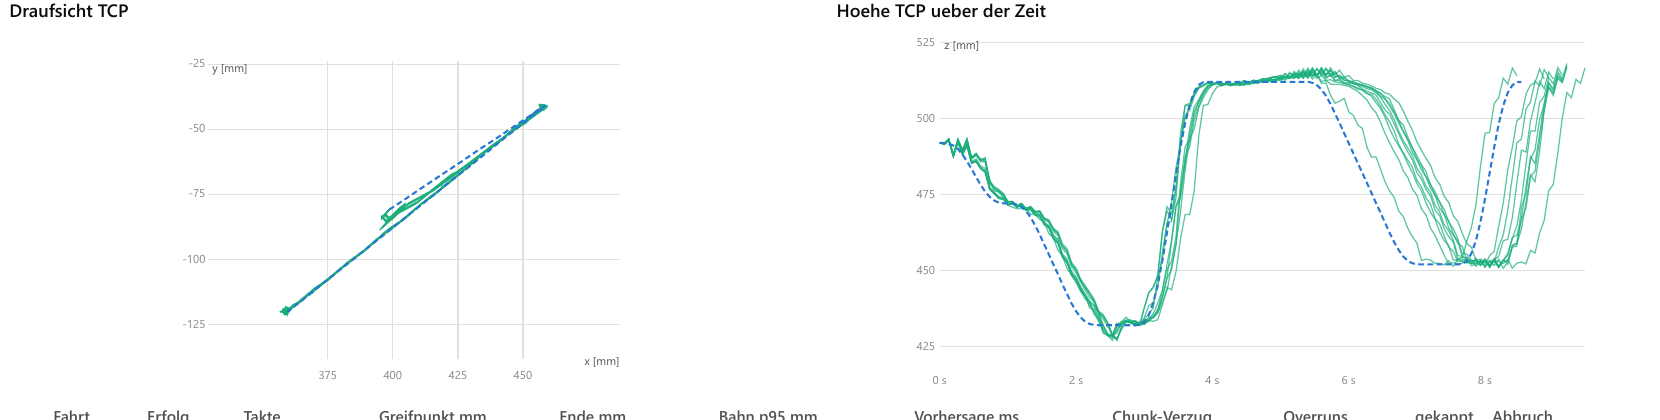
\includegraphics[width=\textwidth]{m4/durchstich_sim_rollouts.png}
  \caption[Fahrten der Policy im Durchstich in der Simulation]{Zehn Fahrten der Policy in
  der Simulation: Draufsicht (links) und Höhe des \acs{tcp} über der Zeit (rechts). Blau
  gestrichelt die ideale Bahn der Aufnahme, grün die Fahrten der Policy.}
  \label{fig:durchstich}
\end{figure}

% ==============================================================================
\section{Inbetriebnahme an der Anlage}
\label{sec:labortage}

An mehreren Labortagen zwischen dem 01.10.\ und dem 21.10.\ wurden die Adapter nach der
Abnahmeliste aus \cref{sec:testkonzept} geprüft. Die wichtigsten Befunde sind bereits in den
jeweiligen Kapiteln beschrieben:
\begin{itemize}
  \item Kinematik der Anlage identisch mit der \ac{vm} (\cref{sec:kinematik}),
  \item abbrechende Bahnen durch einen gedrosselten Rechner und Schleppfehler durch einen zu
    kleinen Override (\cref{sec:sollwerte}),
  \item Zittern bei \code{servo_j} und die Entscheidung für Override \num{0.5}
    (\cref{sec:zittern}),
  \item Kameras nur mit voller Bildrate direkt am Rechner, nicht an einem Verteiler
    (\cref{sec:kameras}).
\end{itemize}
Sechs Aufnahme-Episoden mit der endgültigen Ausführungsart liefen ohne Abbruch; der Arm lag
höchstens \SIrange{0.06}{0.10}{rad} hinter der Sollstellung und damit weit innerhalb der
Grenzen.

% ==============================================================================
\section{Datensätze}
\label{sec:datensaetze}

Ab Ende Oktober wurden an der Anlage Demonstrationen mit echten Bildern aufgenommen
(\cref{tab:datensaetze}). Alle Aufnahmen verwenden \code{servo_j} mit Override \num{0.5},
\SI{15}{\hertz}, beide Kameras und den Transfer mit \SI{0.15}{\metre\per\second}; der Endanflug
lag bis zum 17.11.\ bei \SI{0.05}{\metre\per\second}. Licht (Decke an oder aus, Tageslicht)
und Lage der Draufsichtkamera wurden zwischen den Sitzungen bewusst variiert.

\begin{table}[htbp]
  \centering
  \caption{Aufgenommene Datensätze an der Anlage}
  \label{tab:datensaetze}
  \small
  \begin{tabularx}{\textwidth}{@{}l r X@{}}
    \toprule
    Datensatz & Episoden & Bemerkung \\
    \midrule
    26.10. & 167 & erstes Modell mit echten Bildern \\
    02., 03.\ und 09.11. & 602 & Grundlage der meisten Modelle (\SI{82591}{} Takte, ein Bauteil,
      164 Lagen) \\
    11.11. & 151 & 50 Lagen; 20 davon als feste Testlagen zurückgehalten \\
    ab 19.11. & -- & neuer Datensatz nach den Standards aus \cref{sec:folgerungen} \\
    \bottomrule
  \end{tabularx}
\end{table}

% ==============================================================================
\section{Modellprüfung des Checkpoints vom 09.11.}
\label{sec:modellpruefung}

\paragraph{Frage.} Lernt das Modell auf 602 Episoden, und findet es unbekannte Lagen?

\paragraph{Vorgehen.} Training mit \num{10000} Schritten, Batchgröße 128, in \SI{77}{\minute}.
Danach Stufe~2 in der \ac{vm} (\cref{sec:replay}) an acht unbekannten und drei bekannten Lagen
\quelle{Berichte/2026-11-10_Modellpruefung_Checkpoint_2026-11-09.pdf}.

\paragraph{Ergebnis.}
\begin{itemize}
  \item Der Validierungsverlust sank bis zum Schluss ohne Anzeichen von Überanpassung und lag
    rund fünfmal niedriger als beim Modell vom 26.10. Der mittlere Gelenkfehler betrug
    \SI{0.008}{rad}.
  \item Die offline gemessene Genauigkeit sagt wenig über neue Lagen: Nahe am Greifpunkt
    verrät der Zustand das Ziel bereits, die Bilder werden dort kaum gebraucht.
  \item In der \ac{vm} trafen unbekannte Lagen in der Mitte des Arbeitsraums den Greifpunkt
    auf \SIrange{5}{22}{\milli\metre}, im Median \SI{15}{\milli\metre}. Am fernen Rand
    ($x > \SI{0.5}{\metre}$) gab es reproduzierbare Fehlgriffe um \SIrange{7}{10}{\centi\metre}.
  \item Für Bauteile mit \ang{0} bis \ang{90} Drehung waren die Demonstrationen zur Hälfte um
    \ang{180} gedreht gegriffen; der Griff ist mehrdeutig (\cref{sec:multimodal}).
  \item 6 von 15 Fahrten gingen unter die Tischfläche, bis \SI{56}{\milli\metre}. Der damalige
    Arbeitsraumschutz lag pauschal \SI{145}{\milli\metre} unter dem Tisch und hätte keine davon
    gestoppt. Daraufhin wurde der Tisch aus den Tischpunkten in das Kollisionsmodell und in die
    Modellbeschreibung aufgenommen (\cref{sec:tisch,sec:pruefung-senden}).
\end{itemize}

\begin{figure}[htbp]
  \centering
  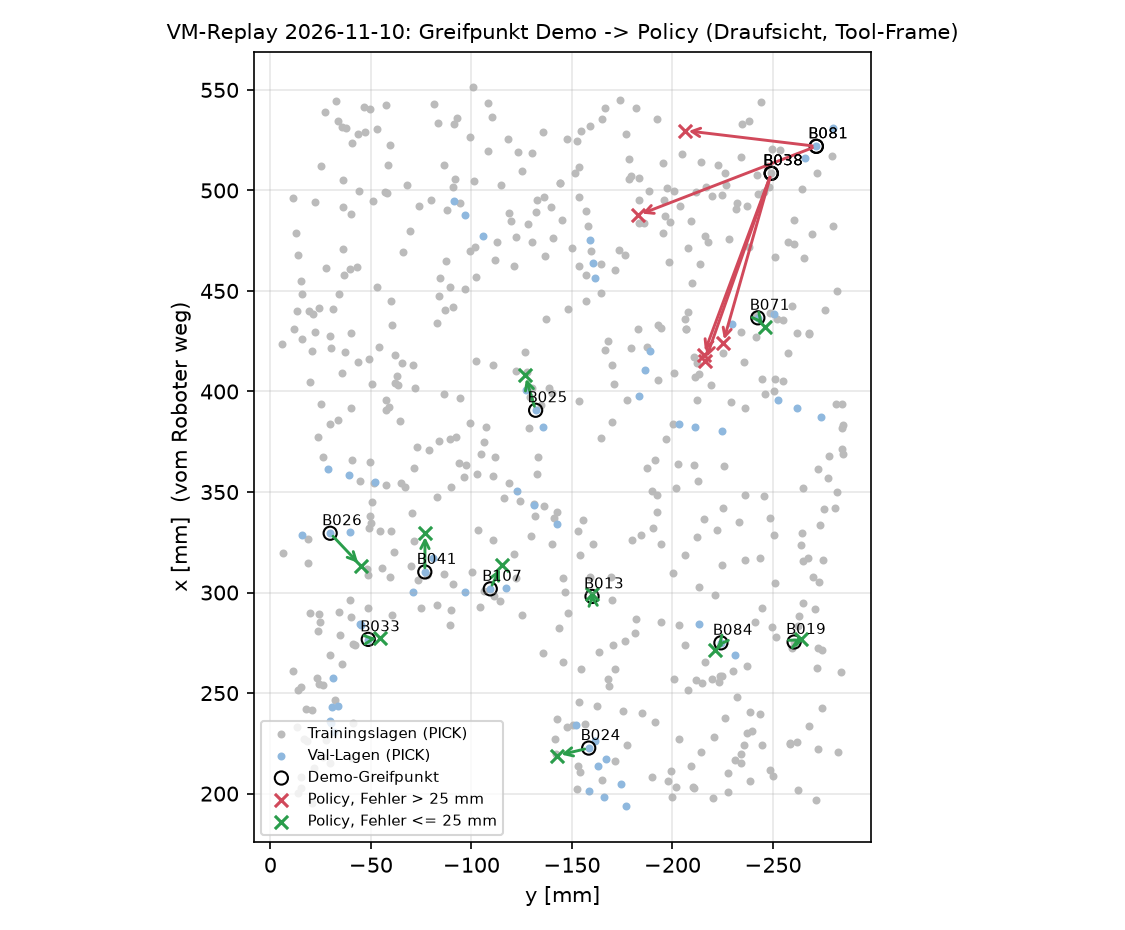
\includegraphics[width=0.85\textwidth]{versuche/modellpruefung_greifpunkte.png}
  \caption[Greifpunkte in der Modellprüfung vom 10.11.]{Greifpunkte der Policy in der
  Modellprüfung vom 10.11.\ (\acs{vm}, Bilder der Aufnahme) gegenüber den Greifpunkten der
  Demonstrationen.}
  \label{fig:modellpruefung}
\end{figure}

% ==============================================================================
\section{VM-Test mit den Aufnahmen vom 11.11.}
\label{sec:replay-1111}

\paragraph{Frage.} Wie verhält sich das Modell an einem Tag, den es nie gesehen hat, und wie
oft würde es in den Tisch fahren?

\paragraph{Vorgehen.} Stufe~1 und Stufe~2 mit allen 151 Episoden vom 11.11.\
\quelle{Berichte/2026-11-13_VM-Replay_Daten-2026-11-11.pdf}.

\paragraph{Ergebnis.} Offline lag der Gelenkfehler je Takt im Median bei \ang{0.7} bis
\ang{1.8}; die Policy ist glatt und genau, wenn Bild und Zustand zusammenpassen. In der \ac{vm}
lag die nächste Annäherung im Median bei \SI{10.7}{\milli\metre}, \SI{49}{\percent} der
Fahrten innerhalb \SI{10}{\milli\metre}, \SI{90}{\percent} innerhalb \SI{39}{\milli\metre}
(\cref{fig:replay-1111}). Ein neuer Tag war damit nicht schlechter als ein Trainingstag, und ein
Unterschied zwischen Licht an und aus war nicht nachweisbar. Zwei Probleme blieben:
\begin{itemize}
  \item In 81 von 151 Fahrten ging die Werkzeugspitze unter die Tischfläche, meist kurz
    \emph{nach} dem Schließen beim seitlichen Wegfahren. Eine Gegenprobe mit Bildwahl nach
    Position statt nach Takt ergab dasselbe; es ist also kein reines Testartefakt.
  \item 22 Fahrten wurden im Transport von der harten Grenze abgebrochen.
\end{itemize}
Die Schwingbahnen in der \ac{vm} stammen überwiegend aus dem Testverfahren selbst: Die
Bilder zeigen die verrauschte Bahn der Aufnahme, der Arm ist aber woanders, und die Policy
korrigiert Abweichungen, die es nicht gibt.

\begin{figure}[htbp]
  \centering
  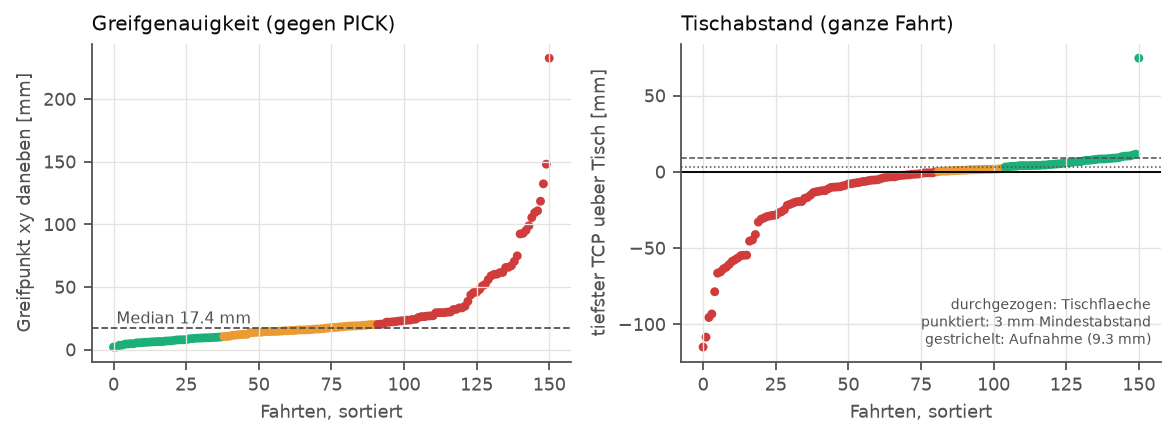
\includegraphics[width=\textwidth]{versuche/replay_fehler_tisch.png}
  \caption[VM-Test mit den Aufnahmen vom 11.11.]{VM-Test mit den Aufnahmen vom 11.11.\
  (151 Fahrten, sortiert). Links der waagerechte Abstand zum Greifpunkt beim Schließen, rechts
  der tiefste Punkt des \acs{tcp} über der Tischfläche.}
  \label{fig:replay-1111}
\end{figure}

% ==============================================================================
\section{Versuchsreihe Policy-Varianten}
\label{sec:varianten}

\paragraph{Frage.} Lassen sich die Probleme aus \cref{sec:replay-1111} mit den vorhandenen
Daten beheben? Jede Maßnahme wurde einzeln gemessen
\quelle{Berichte/Versuchsreihe_Policy-Varianten/}.

\paragraph{Vorgehen.} Aus den 50 Lagen vom 11.11.\ wurden 20 als feste Testlagen gewählt und
aus allen Trainingsdaten herausgenommen; getestet wurde mit ihren 59 Episoden in der \ac{vm}.
Jede Variante unterscheidet sich von der Basis~A in genau einer Änderung und wurde mit
\num{10000} Schritten trainiert (\cref{tab:varianten-def}). Ausgewertet wurde paarweise je
Testlage mit Vorzeichentest. Zwei Durchläufe desselben Modells streuten bei Annäherung und
Tisch um etwa \SI{\pm 1.5}{\milli\metre} und \SI{\pm 3}{Prozentpunkte}, bei Abbrüchen und
Endstellung um bis zu \SI{18}{Prozentpunkte}; diese beiden Werte sind nur bei großen
Unterschieden deutbar.

\begin{table}[htbp]
  \centering
  \caption{Varianten der Versuchsreihe}
  \label{tab:varianten-def}
  \small
  \begin{tabularx}{\textwidth}{@{}l X X@{}}
    \toprule
    Variante & Änderung & prüft \\
    \midrule
    I & nur Ausführung: stärkere Gewichtung neuer Folgen, seltenere Neuvorhersage & Mitteln der
      Folgen \\
    A Basis & alle Daten ohne Testlagen (694 Episoden) & Bezugspunkt \\
    B Pause kurz & Stillstand am Greifpunkt von 8 auf 3 Takte gekürzt & Mehrdeutigkeit am
      Greifpunkt \\
    C Nur Griff & Episode endet 3 Takte nach dem Schließen; Transport plant der Planer &
      Aufteilung der Aufgabe \\
    D Eine Drehung & um \ang{180} gedrehte Griffe entfernt (529 Episoden) & mehrdeutige
      Greifdrehung \\
    C$'$ (später C2) & wie C, aber ohne die Daten vom 11.11.\ (602 Episoden) & Effekt der
      Daten vom 11.11. \\
    F & wie A, mit Helligkeits- und Farbaugmentierung & Lichtunterschiede \\
    \bottomrule
  \end{tabularx}
\end{table}

\begin{table}[htbp]
  \centering
  \caption[Ergebnisse der Versuchsreihe in der VM]{Ergebnisse der Versuchsreihe in der
  \acs{vm} (59 Fahrten je Modell, Bilder der Testlagen). \enquote{alt}: Checkpoint vom 09.11.,
  ohne Daten vom 11.11.}
  \label{tab:varianten}
  \small
  \begin{tabular}{@{}l r r r r r r@{}}
    \toprule
    Modell & Annäh. & $\le$\SI{10}{mm} & beim Schließen & unter Tisch & Abbruch & Endst. \\
    \midrule
    alt, Seed 0 & \SI{10.2}{mm} & \SI{50}{\percent} & \SI{18.6}{mm} & \SI{54}{\percent} & \SI{32}{\percent} & \SI{41}{\percent} \\
    alt, Seed 1 & \SI{10.6}{mm} & \SI{50}{\percent} & \SI{18.0}{mm} & \SI{59}{\percent} & \SI{36}{\percent} & \SI{59}{\percent} \\
    A & \SI{15.3}{mm} & \SI{28}{\percent} & \SI{28.4}{mm} & \SI{58}{\percent} & \SI{25}{\percent} & \SI{64}{\percent} \\
    B & \SI{15.6}{mm} & \SI{32}{\percent} & \SI{20.8}{mm} & \SI{46}{\percent} & \SI{29}{\percent} & \SI{59}{\percent} \\
    C & \SI{17.5}{mm} & \SI{20}{\percent} & \SI{23.2}{mm} & \SI{36}{\percent} & \SI{14}{\percent} & \SI{85}{\percent} \\
    D & \SI{16.6}{mm} & \SI{33}{\percent} & \SI{26.8}{mm} & \SI{59}{\percent} & \SI{36}{\percent} & \SI{61}{\percent} \\
    C$'$ & \SI{15.5}{mm} & \SI{32}{\percent} & \SI{18.7}{mm} & \SI{47}{\percent} & \SI{7}{\percent} & \SI{90}{\percent} \\
    F & \SI{14.9}{mm} & \SI{29}{\percent} & \SI{26.9}{mm} & \SI{63}{\percent} & \SI{34}{\percent} & \SI{39}{\percent} \\
    \bottomrule
  \end{tabular}
\end{table}

\paragraph{Ergebnisse.}
\begin{enumerate}
  \item \textbf{Ausführung (I):} Weniger Mitteln machte die Fahrt in fast allen Kennzahlen
    schlechter, unruhiger und tiefer. Die Standardeinstellung blieb.
  \item \textbf{Daten vom 11.11.:} Alle Varianten mit diesen Daten trafen schlechter als der
    alte Checkpoint (A auf 17 von 20 Lagen, $p = 0{,}001$). Ein zweites Training mit anderem
    Startwert zeigte, dass die Streuung zwischen Trainings klein ist. Eine Ursache in den Daten
    wurde nicht gefunden: Bahnform, Rauschen, Synchronisation und Kameralage waren an allen
    Tagen gleich; auffällig war nur deutlich mehr Tageslicht. Auch Licht-Augmentierung (F)
    änderte daran nichts. Die Ursache ist offen.
  \item \textbf{Kurze Pause (B):} weniger Tischfahrten, Genauigkeit unverändert.
  \item \textbf{Nur Griff (C, C$'$):} Den Transport dem Planer zu überlassen, senkt
    Tischfahrten und Abbrüche deutlich und lässt fast alle Fahrten durchlaufen. Ohne die
    Daten vom 11.11.\ (C$'$) ist die Genauigkeit beim Schließen so gut wie beim alten
    Checkpoint; die Abbrüche sinken von \SIrange{32}{36}{\percent} auf \SI{7}{\percent}.
  \item \textbf{Eine Drehung (D):} kein Gewinn, aber 165 Demonstrationen weniger.
\end{enumerate}
C$'$ wurde damit das Modell für den ersten Anlagentest (\enquote{C2}). Seitdem endet die
Aufgabe der Policy mit dem Griff, und der Transport zum Übergabepunkt ist geplant.

\todo[inline]{Die Aufteilung \enquote{Policy greift, Planer transportiert} in
\cref{ch:einleitung,ch:integration} nachziehen, sobald sie für den Betrieb endgültig ist. Der
Aufruf aus dem Ablauf (\texttt{m4\_grasper.py}) nutzt den geplanten Transport noch nicht.}

% ==============================================================================
\section{Anlagentest mit C2}
\label{sec:anlagentest-c2}

\paragraph{Frage.} Wie genau trifft die Policy an der realen Anlage?

\paragraph{Vorgehen.} Probegriff mit bekannter Lage (\cref{sec:erfolg}) an fünf Lagen, neun
Fahrten. Die Policy fuhr selbst an und wurde kurz über dem Bauteil angehalten; aus dem Rest
ihrer Vorhersage wurde bestimmt, wo sie gegriffen hätte. Danach korrigierte der Planer auf den
Greifpunkt, griff und legte an einer neuen Lage ab
\quelle{Berichte/2026-11-16_Anlagentest_var_C2.pdf}.

\paragraph{Ergebnis.} Der vorhergesagte Greifpunkt lag im Median \SI{8.7}{\milli\metre}
daneben (\SIrange{1.0}{18.0}{\milli\metre}); 5 von 8 Probegriffen lagen innerhalb
\SI{10}{\milli\metre}. Das passt zum \ac{vm}-Test (\SI{10.7}{\milli\metre}). Der Drehfehler
lag meist unter \ang{5}. \Cref{fig:c2-versatz} zeigt, wo der Fehler entsteht: Bis
\code{PRE_PICK} folgt die Policy der senkrechten Bahn auf \SIrange{1}{7}{\milli\metre};
darunter zögert sie und driftet innerhalb weniger Takte \SIrange{10}{29}{\milli\metre} zur
Seite. Genau diese Zustände kommen in den Demonstrationen nicht vor, weil dort der Trichter
das Rauschen auf null gedämpft hat. Das war der Anlass für den gezielten Versatz im Anflug
(\cref{sec:versatz}) und für \ac{dagger} (\cref{ch:fazit}).

\begin{figure}[htbp]
  \centering
  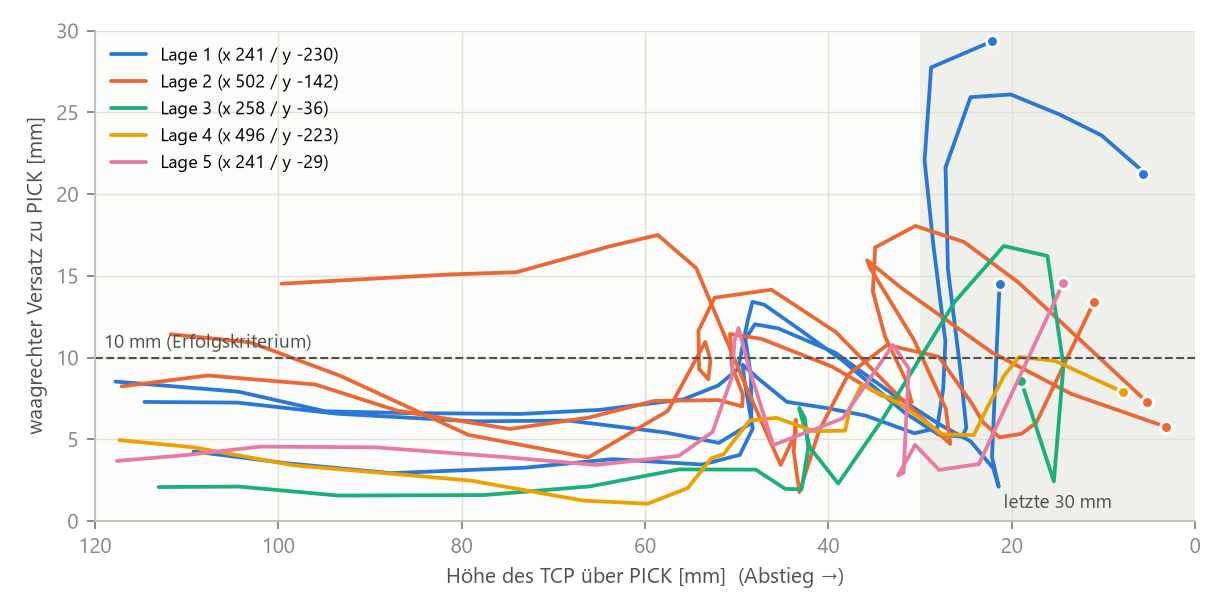
\includegraphics[width=\textwidth]{versuche/c2_versatz_hoehe.png}
  \caption[Seitlicher Versatz über der Höhe im Anlagentest]{Waagerechter Abstand des
  gemessenen \acs{tcp} zum Greifpunkt über der Höhe, je Fahrt im Anlagentest vom 16.11.\
  (Farbe: Lage, Punkt: Stopp).}
  \label{fig:c2-versatz}
\end{figure}

\paragraph{Auffälligkeiten.} Zweimal wurde der Not-Halt am Bedienhandgerät gedrückt, weil der
Arm abzutauchen schien. Die Ausführung bemerkte das nicht und sendete weiter Ziele. Daraus
entstand die Überwachung auf einen stehenden Arm (\cref{sec:ueberwachung}). Ob die Policy
selbst richtig schließt, blieb ungeprüft, weil jede Fahrt vor dem Schließen angehalten wurde.

% ==============================================================================
\section{Empfindlichkeit gegenüber der Kameralage}
\label{sec:kamera-empfindlichkeit}

\paragraph{Frage.} Würde eine Rektifizierung der Draufsicht über die ArUco-Marker helfen?

\paragraph{Vorgehen.} Offline wurden für 30 Episoden (davon 15 von einem Tag, der nicht im
Training war) die Bilder gezielt gestört und die Änderung der Vorhersage gemessen, bei
gleichem Diffusionsrauschen \quelle{Berichte/2026-11-16_Kameraempfindlichkeit_var_C2.pdf}.

\paragraph{Ergebnis} (\cref{fig:kamera}):
\begin{itemize}
  \item Eine Verschiebung der Draufsicht um \SI{10}{Pixel}, was einem um etwa
    \SI{3}{\centi\metre} verschobenen Bauteil entspricht, ändert die Vorhersage nur um
    \SIrange{0.6}{1.5}{\milli\metre}; eine Drehung um \ang{5} um \SIrange{1.0}{1.7}{\milli\metre}.
    Vermutlich hat der zufällige Bildausschnitt im Training diese Unempfindlichkeit erzeugt.
  \item Die Draufsicht wird vor allem im Anflug gebraucht (ausgeblendet
    \SIrange{12}{13}{\milli\metre} Änderung), am Griff zählt die Handgelenkkamera (ausgeblendet
    bis \SI{18}{\milli\metre}).
  \item Offline liegt die Vorhersage in den letzten \SI{20}{\milli\metre} auch am neuen Tag nur
    \SIrange{2.2}{2.4}{\milli\metre} von der Aufnahme entfernt. Die \SI{8.7}{\milli\metre} an der
    Anlage entstehen also im geschlossenen Kreis, in Zuständen, die die Policy selbst
    herbeiführt, und nicht durch ein anders aussehendes Bild.
\end{itemize}
Die Rektifizierung lohnt sich damit nicht; die Entscheidung aus \cref{sec:kameras} wurde
bestätigt. Wichtiger ist eine stabile Handgelenkkamera mit gleichbleibendem Licht.

\begin{figure}[htbp]
  \centering
  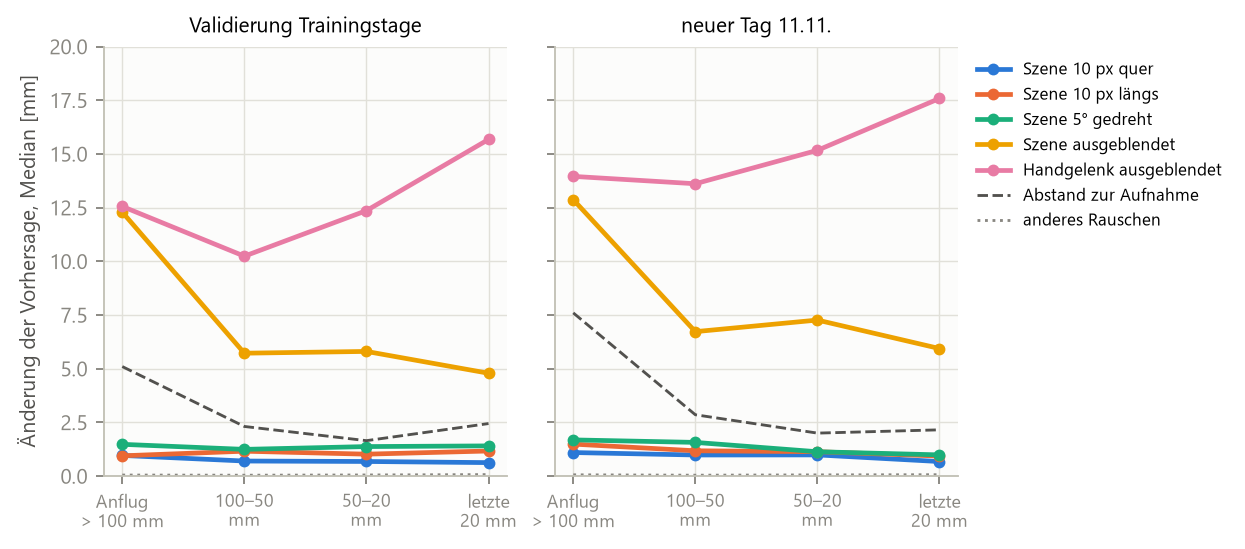
\includegraphics[width=\textwidth]{versuche/kamera_empfindlichkeit.png}
  \caption[Empfindlichkeit der Policy gegenüber Bildstörungen]{Änderung der Vorhersage
  (Median) je Phase der Fahrt und Art der Bildstörung.}
  \label{fig:kamera}
\end{figure}

% ==============================================================================
\section{Drehbias der Demonstrationen}
\label{sec:drehbias}

\paragraph{Frage.} An der Anlage drehte C2 bei Lagen, die eine Drehung nach minus verlangen,
im Median \ang{31} zu wenig (8 Fahrten), bei Plus-Lagen nur \ang{3}. Woran liegt das?

\paragraph{Vorgehen.} Auswertung der Drehungen in den Demonstrationen und zwei Varianten mit
denselben Daten: C3 zieht Minus-Episoden im Training \num{2.83}-mal häufiger, C3a lässt
238 Plus-Episoden weg. Vergleich offline an den Anlagensituationen und in der \ac{vm}
\quelle{Berichte/2026-11-17_Drehbias_C3.pdf}.

\paragraph{Ergebnis.}
\begin{itemize}
  \item Die Demonstrationen waren einseitig: \SI{62}{\percent} Plus-, \SI{25}{\percent}
    Minus-Drehungen, im Mittel \ang{+38.8} (\cref{fig:drehbias}). Ursache war die
    Verteilung der Drehung um die geteachte Lage statt um die Startstellung
    (\cref{sec:lagen}).
  \item Gewichten (C3) wirkt besser als Ausdünnen (C3a): C3 will bei Minus-Lagen im Median
    \ang{15} mehr drehen, C3a nur \ang{9} und verliert durch die fehlenden Daten an
    Genauigkeit.
  \item Der Bias ist nur ein Teil der Ursache. Die ganze Drehung geschieht in der Gelenkfahrt
    bis \code{ANFLUG}; darunter dreht keine Demonstration mehr, und die Policy holt fehlende
    Drehung nicht nach. Außerdem kommandiert sie etwa \SI{35}{\percent} größere Schritte als
    die Demonstrationen, und der Arm folgt schlechter.
  \item Keiner der Tests ohne Anlage koppelt die Bilder an die Bewegung zurück; keiner konnte
    den Drehfehler deshalb zuverlässig vorhersagen.
\end{itemize}

\begin{figure}[htbp]
  \centering
  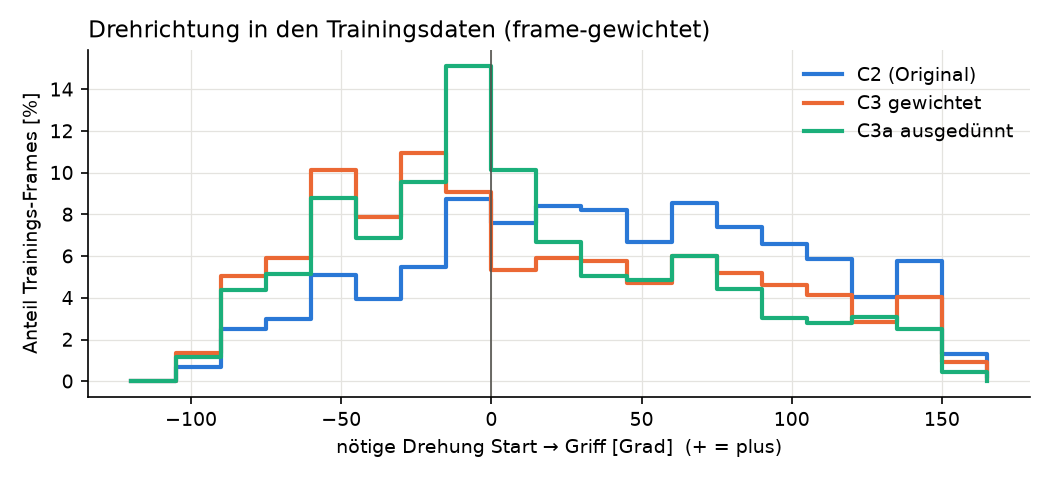
\includegraphics[width=0.85\textwidth]{versuche/drehbias_verteilung.png}
  \caption[Verteilung der Drehungen in den Demonstrationen]{Verteilung der nötigen Drehung
  zwischen Start und Griff in den 602 Demonstrationen.}
  \label{fig:drehbias}
\end{figure}

% ==============================================================================
\section{Folgerungen für den neuen Datensatz}
\label{sec:folgerungen}

Aus den Versuchen bis zum 17.11.\ wurden die Standards für den nächsten Datensatz abgeleitet
und im Code umgesetzt:
\begin{itemize}
  \item Drehung der Lagen um die Startstellung verteilt (Drehbias),
  \item Endanflug \SI{0.02}{\metre\per\second} (mehr Bilder kurz vor dem Bauteil),
  \item gezielter seitlicher und Drehversatz im Anflug (Zögern und Abdriften unter
    \code{PRE_PICK}, \cref{sec:versatz}),
  \item Kameralicht an der Handgelenkkamera und fester Weißabgleich,
  \item erste Lage aus der Objekterkennung von Modul~1,
  \item Aufnahme nur bis zum Griff (Ablauf \code{pick_bis_griff}, seit 19.11.): Nach dem Griff
    hebt der Arm an und fährt an einen gemeinsamen Endpunkt \SI{15}{\centi\metre} über der
    Tischmitte statt zur Prüfvorrichtung. Das folgt aus dem Ergebnis von C und C$'$, spart Zeit
    je Episode und beim Zurücklegen. Der Endpunkt muss für alle Lagen gleich sein, damit die
    Rückfahrt zur nächsten Lage passt. Bei der Ausführung plant dann der Planer den Transport
    zum Übergabepunkt.
\end{itemize}

% ==============================================================================
\section{Weitere Versuche}
\label{sec:weitere-versuche}

\todo[inline]{Platz für die Ergebnisse mit dem neuen Datensatz (ab 19.11.), den Gegenversuch
mit C3 an der Anlage und \acs{dagger}.}
